\documentclass[a4paper, 12pt]{report}
\usepackage{graphicx}
\usepackage[utf8]{inputenc}
\usepackage{graphicx}
\usepackage{fancyhdr}
\usepackage[french]{babel}
\usepackage{listings}
\usepackage{titlesec}

\newcommand{\myparagraph}[1]{\paragraph{#1}\mbox{}\newline\\}

\titleformat{\subparagraph}
    {\normalfont\normalsize\bfseries}{\thesubparagraph}{1em}{}
\titlespacing*{\subparagraph}{\parindent}{3.25ex plus 1ex minus .2ex}{.75ex plus .1ex}

\title{Rapport de Stage}
\author{Pierre De Abreu}
\date{08 Février 2016 - 08 Aout 2016}

\newcommand{\HRule}{\rule{\linewidth}{0.5mm}}
 
\pagestyle{fancy}
\fancyhf{}
\rhead{Sogeti, ESEC}
\lhead{EPITA / SRS 2016}
\rfoot{
\includegraphics[width=1cm, height=1cm]{images/esec-footer.png}}
\lfoot{
\includegraphics[width=2cm]{images/epita.png}}
\lfoot{
\includegraphics[width=2cm]{images/srs.png}}
\cfoot{\thepage}
 
\begin{document} 
\lstset{language=python}
\begin{titlepage}
\begin{center}

% Upper part of the page. The '~' is needed because \\
% only works if a paragraph has started.

\includegraphics[width=0.3\textwidth]{images/epita.png}~\\[1cm]

\textsc{\LARGE EPITA}\\[1.5cm]

\textsc{\Large Stage de fin d'étude - Annexes}\\[0.5cm]
\textsc{\Large 08/02/2016 - 08/08/2016}

% Title
\HRule \\[0.4cm]
{ \huge \bfseries Sogeti, ESEC \\[0.4cm] }

\HRule \\[1.5cm]

% Author and supervisor
\begin{minipage}{0.4\textwidth}
\begin{flushleft} \large
\emph{Auteur:}\\
Pierre \textsc{De Abreu}
\end{flushleft}
\end{minipage}
\begin{minipage}{0.4\textwidth}
\begin{flushright} \large
\emph{Maitre de stage:} \\
Adrien \textsc{Fay}
\end{flushright}
\end{minipage}


\includegraphics[width=0.3\textwidth]{images/esec.png}~\\[1cm]

\vfill

% Bottom of the page
{\large Recherche de vulnérabilité (Use-After-Free)\paragraph{}}
{\large 21 Juillet 2016}

\end{center}
\end{titlepage}

\begin{large}
\thispagestyle{empty}
\tableofcontents
\end{large}
\setcounter{page}{0}

\part{Documentation sur les logiciels}
\chapter{Miasm}
\begin{figure}[h]
    \centering
    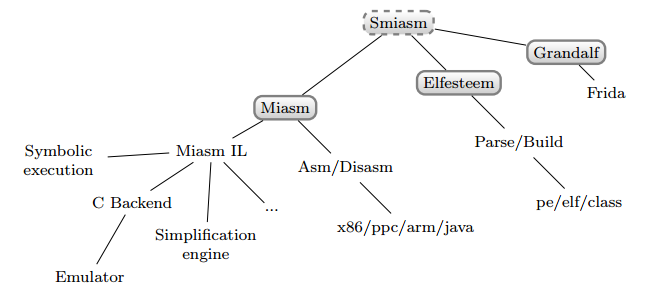
\includegraphics[scale=0.5]{images/miasm-orga.png}
    \caption{Composants de miasm.}
    Architecture de l'outil Miasm\footnote{https://www.sstic.org/media/SSTIC2012/SSTIC-actes/miasm\_framework\_de\_reverse\_engineering/SSTIC2012-Article-miasm\_framework\_de\_reverse\_engineering-desclaux\_1.pdf}.
\end{figure}

\part{Résultats bruts}
\chapter{Sortie du programme}
\begin{figure}[h]
    \centering
    \includegraphics[scale=0.5]{images/tracking-set.png}
    \caption{Représentation de l'attribut tracking\_set (affichage de debug).}
    Chaque emplacement est associé à un identifiant d'allocation.
\end{figure}
\begin{figure}[h]
    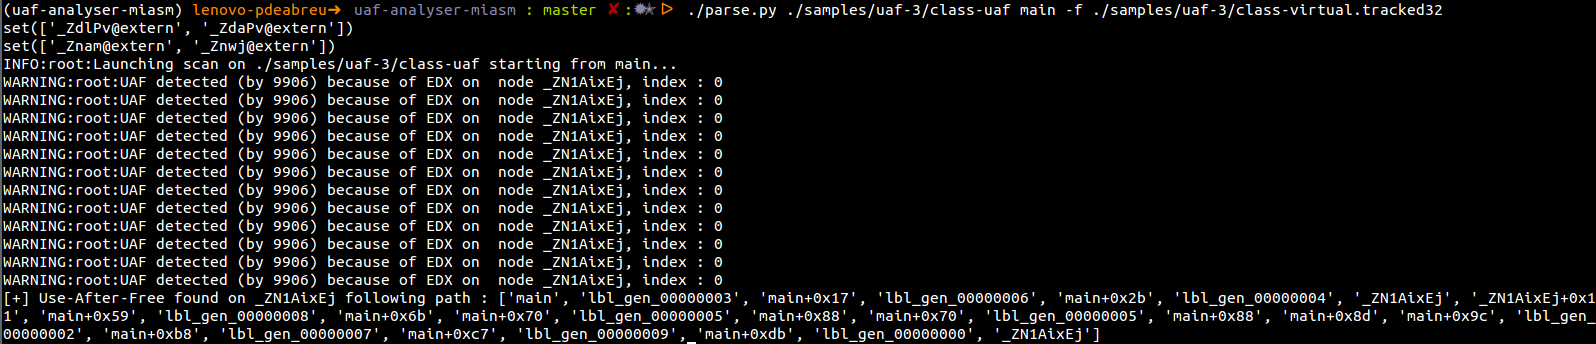
\includegraphics[height=8cm]{images/output-samples.png}
    \caption{Sortie complète d'un test.}
    Chaque résultat positif est décomposé comme suit:
    \begin{itemize}
        \item (by XXXX) donne le PID du processus ayant découvert la vunérabilité.
        \item Le registre ou emplacement mémoire lu coupable.
        \item Le noeud du graphe sur lequel le résultat a lieu.
        \item L'indicateur d'allocation de la zone mémoire utilisée.
    \end{itemize}
    A la fin du programme, chaque chemin positif est donné en sortie.
\end{figure}

\begin{figure}[h]
    \centering
    \begin {lstlisting}[frame=single]
allocation:
g_malloc0@extern
g_malloc0_n@extern
g_malloc@extern
g_malloc_n@extern
free:
g_free@extern
    \end{lstlisting}
    \caption{Fonction traquées pour le logiciel evince. }
    Fichier de configuration contenant les fonctions traquées pour le logiciel
evince sous Linux (Ubuntu 14.10).
\end{figure}

\chapter{Graphes}

\begin{figure}[h]
    \centering
    \begin {lstlisting}[frame=single]
int *global = NULL;

static void e(void) {
    printf("Test.\n");
}

static void g(int fd, int fd2, int fd3) {
    close(fd);
    for (int i = 0; i < (fd + fd2 + fd3); i ++)
        e();
}

void f(void) {
    int fd = open("file", O_RDONLY);
    g(fd, fd + 1, fd + 2);
    int a = a + 1;
    int *b = malloc(sizeof(int));
    int *i = malloc(sizeof(int));
    for (int i = 0; i < 10; i++) {
        printf("foo : %p\n", b);
        a += 2;
    }
    free(b);
    int *c = i;
    int *d = i;
    global = d;
    printf("%d%s%p", a, "f\n", c);
    printf("%d%s%p", a, "f\n", d);
    printf("%d%s%p", a, "f\n", global);
}

int main(void)
{
    while (1) {
      for (int i = 0; i < 50; i++) {
            if (malloc(sizeof(int)))
                f();
            else
                g(i, i+1, i+2);
      }
    }
    return 0;
}
    \end{lstlisting}
    \caption{Programme 1.}
\end{figure}


\begin{figure}[h]
    \centering
    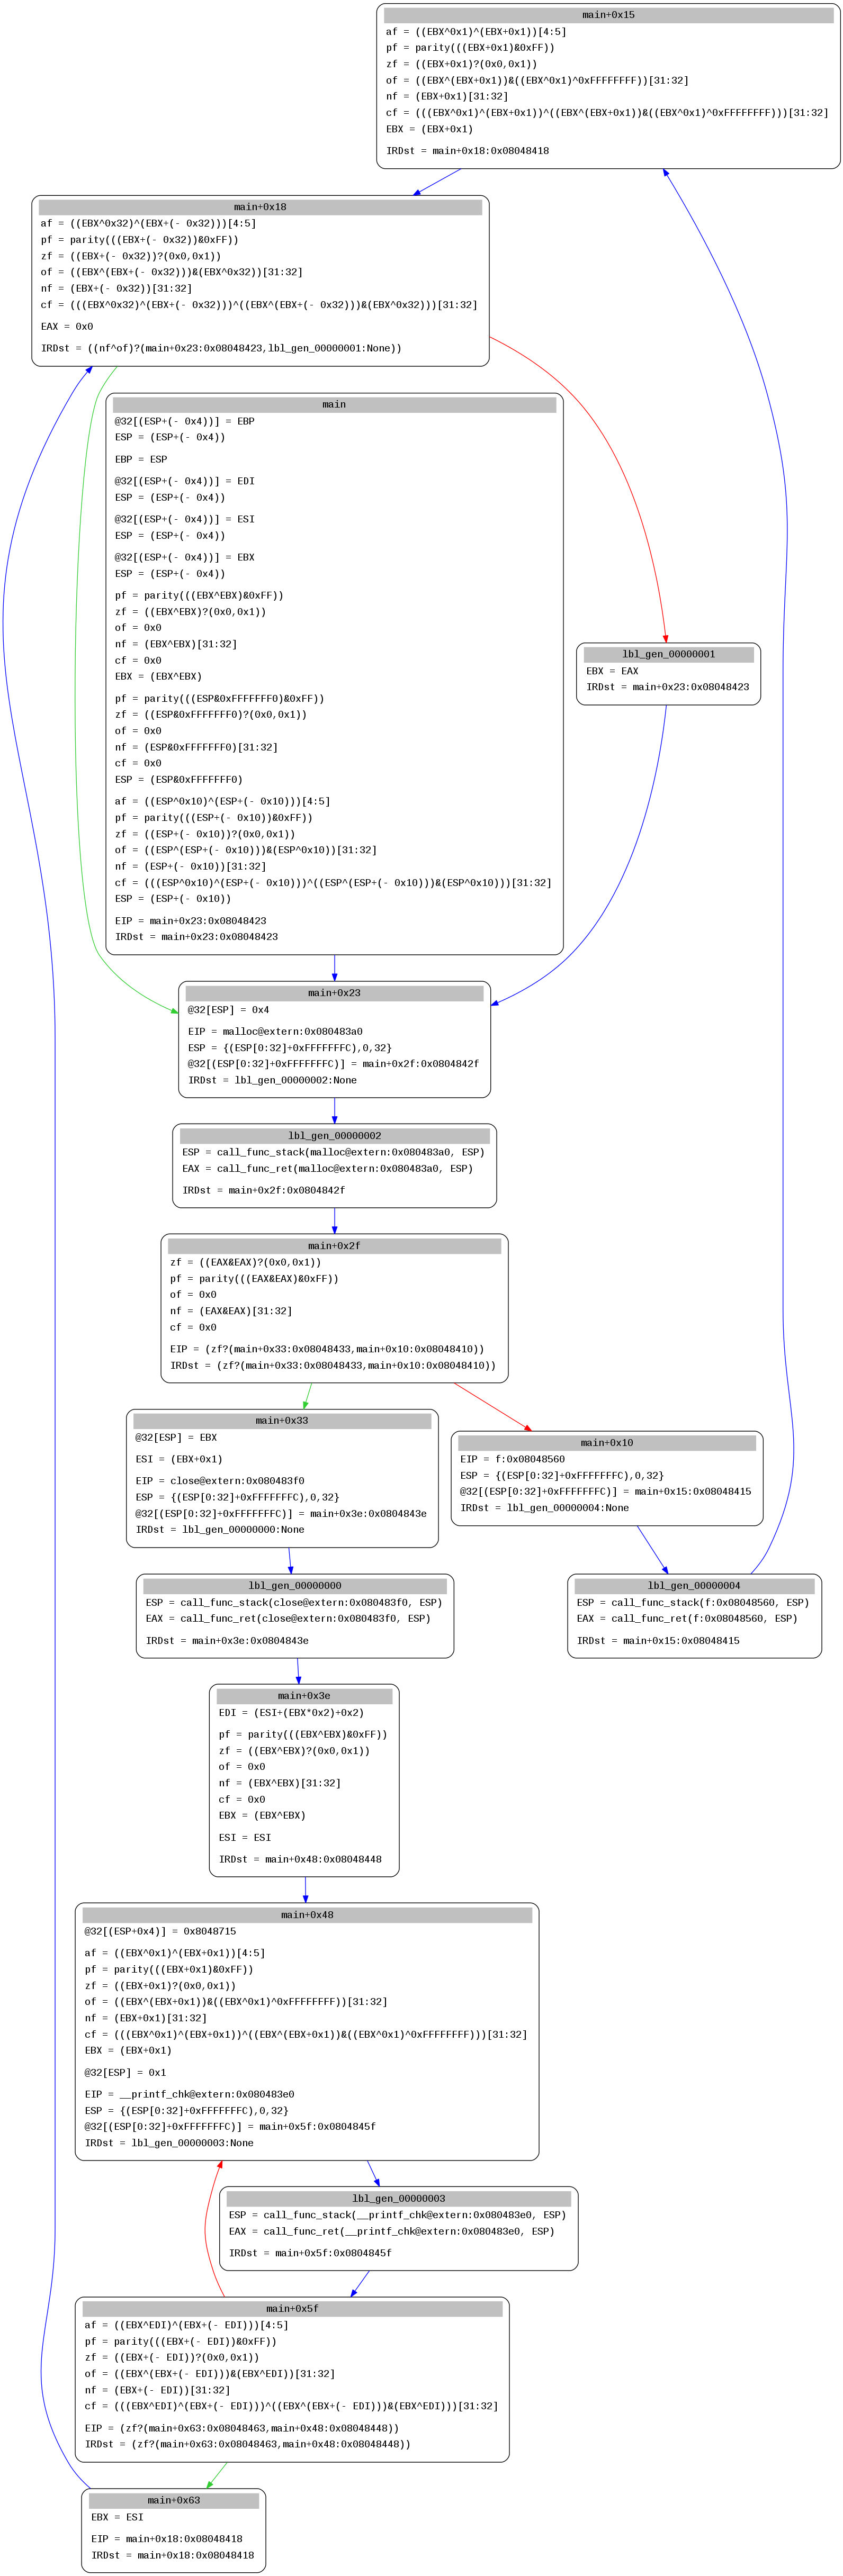
\includegraphics[scale=0.125]{images/simple-graph.png}
    \caption{Graphe associé au programme 1}
\end{figure}

\chapter{Convention d'appel}

\begin{figure}[h]
    \centering
    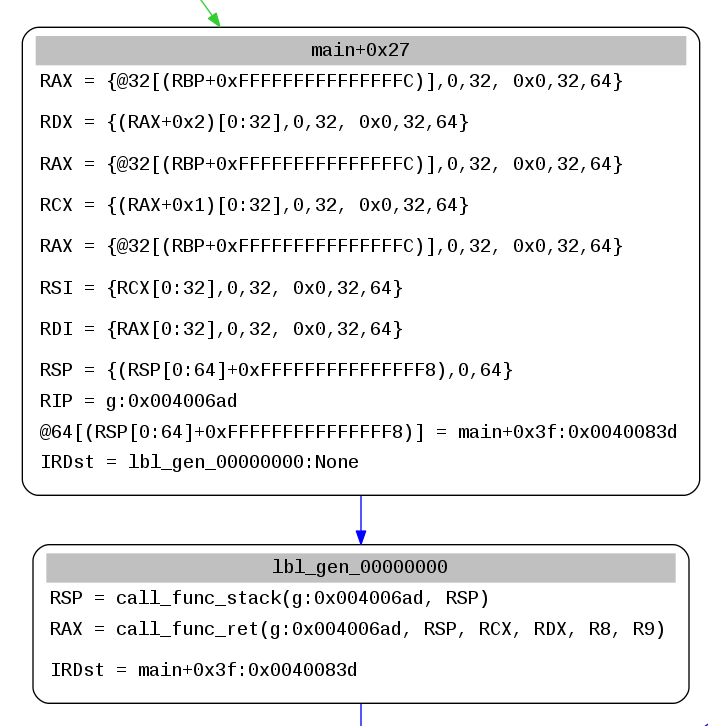
\includegraphics[scale=0.5]{images/main.png}
    \caption{Appel d'une fonction sur SystemV 64 bits.}
    Les registres suffisent aux arguments.
\end{figure}
\begin{figure}[h]
    \centering
    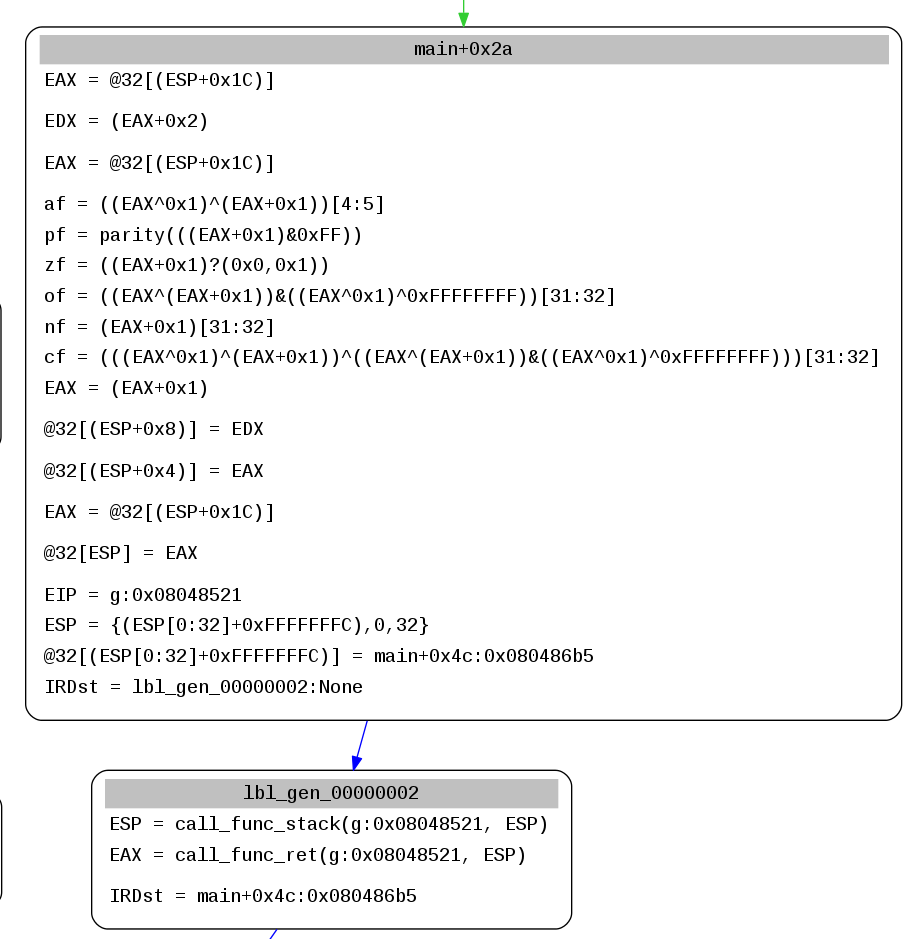
\includegraphics[scale=0.5]{images/main32.png}
    \caption{Appel d'une fonction sur SystemV 32 bits.}
    Les arguments sont passé sur la pile. La différence avec les autres placements
sur la pile est l'offset positif.
\end{figure}

%\begin{figure}[h]
%    \centering
%    \includegraphics[scale=0.001]{tracking-set.png}
%    \caption{Graphe d'un petit projet de première année du cyle ingénieur.}
%\end{figure}


\begin{large}
\thispagestyle{empty}
\listoffigures
.
\end{large}

\end{document}
